\section{Theoretical Analysis}
\label{sec:analysis}

In this section, the circuit shown in \textbf{Figure~\ref{fig:diagram_t3}} is analysed
theoretically.
\begin{figure}[H] \centering
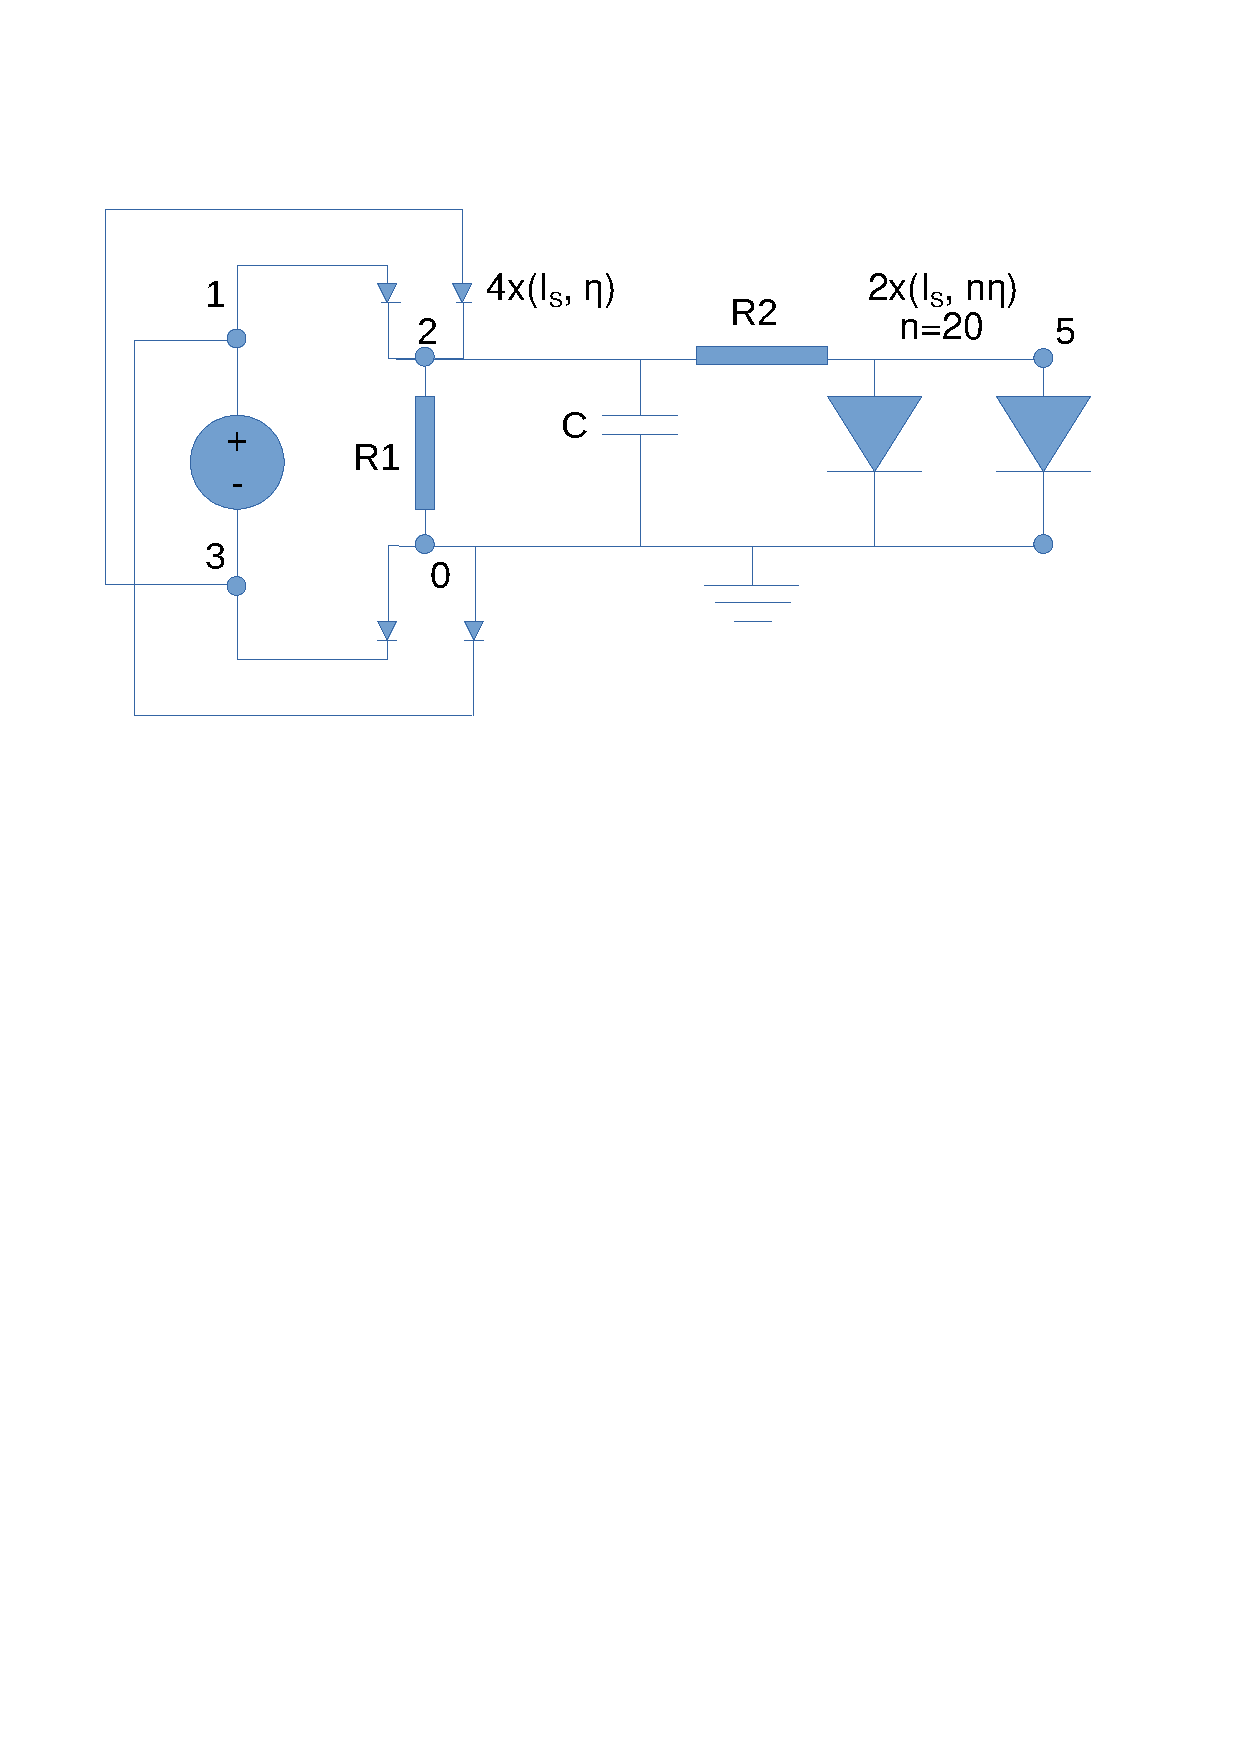
\includegraphics[width=0.6\linewidth]{diagram_t3.pdf}
\vspace{-6cm}
\caption{Diagram of the circuit considered for the computations and simulations}
\label{fig:diagram_t3}
\end{figure}

The transformer used has an n:1 ratio. This means that the initial voltage source will have it's Amplitude (A) reduced by a factor of n. Therefore we can represent the voltage at the terminals of the transformer as a voltage source with an Amplitude of A/n and with the same frequency as the initial source. 

The output of the transformer will be the input of our Envelope detector.The Envelope detector circuit is made up of a rectifier and a capacitor.The rectifier is a full-wave bridge rectifier circuit and is composed of 4 diodes and a resistor. The full-wave rectifier was used as oposed to a half-wave rectifier because the full-wave rectifier allows us to reduce the ripple without incrising the time constant which will avoid a big raise in costes. The full-wave rectifier reduces the ripple because the voltage that comes out of the transformer will leave the rectifier oscillating at twice the frequency and with less amplitude, which helps us in our ripple problem.

The output of the Envelope Detector will be the input of the Voltage Regulator. The voltage regulator is made up of 40 diodes and one resistence. The resistende is in series with a paralel of 2 rows of 20 diodes each. The diodes in each row are in series. The output of the paralel of diodes is the output of the AC/DC converter.

In the Envolope Detector the diode model used has an ideal diode and an voltage source while in the Voltage regulator de Diode model has a ideal diode, a voltage source and a resistor. 

The ratio of the transformer and the values of the resistors, the capacitor nº of diodes are the following:\\
$ n_{transformer} = 5.48:1 $  \\
$ R_{env} = 100 kohm$  \\
$ C_{env} = 100 uF$  \\
$ R_{reg} = 120 kohm$  \\
$ n_{diodes} = 40 $   \\
%point 1


%In \textbf{Table~\ref{tab:theoretical}} the values for the branch currents and the node voltages obtained from the Octave script for both methods are presented. Here, the node voltages in the mesh method were computed from the respective currents, which were determined as described in the previous subsection.





%\begin{figure}[H] \centering
%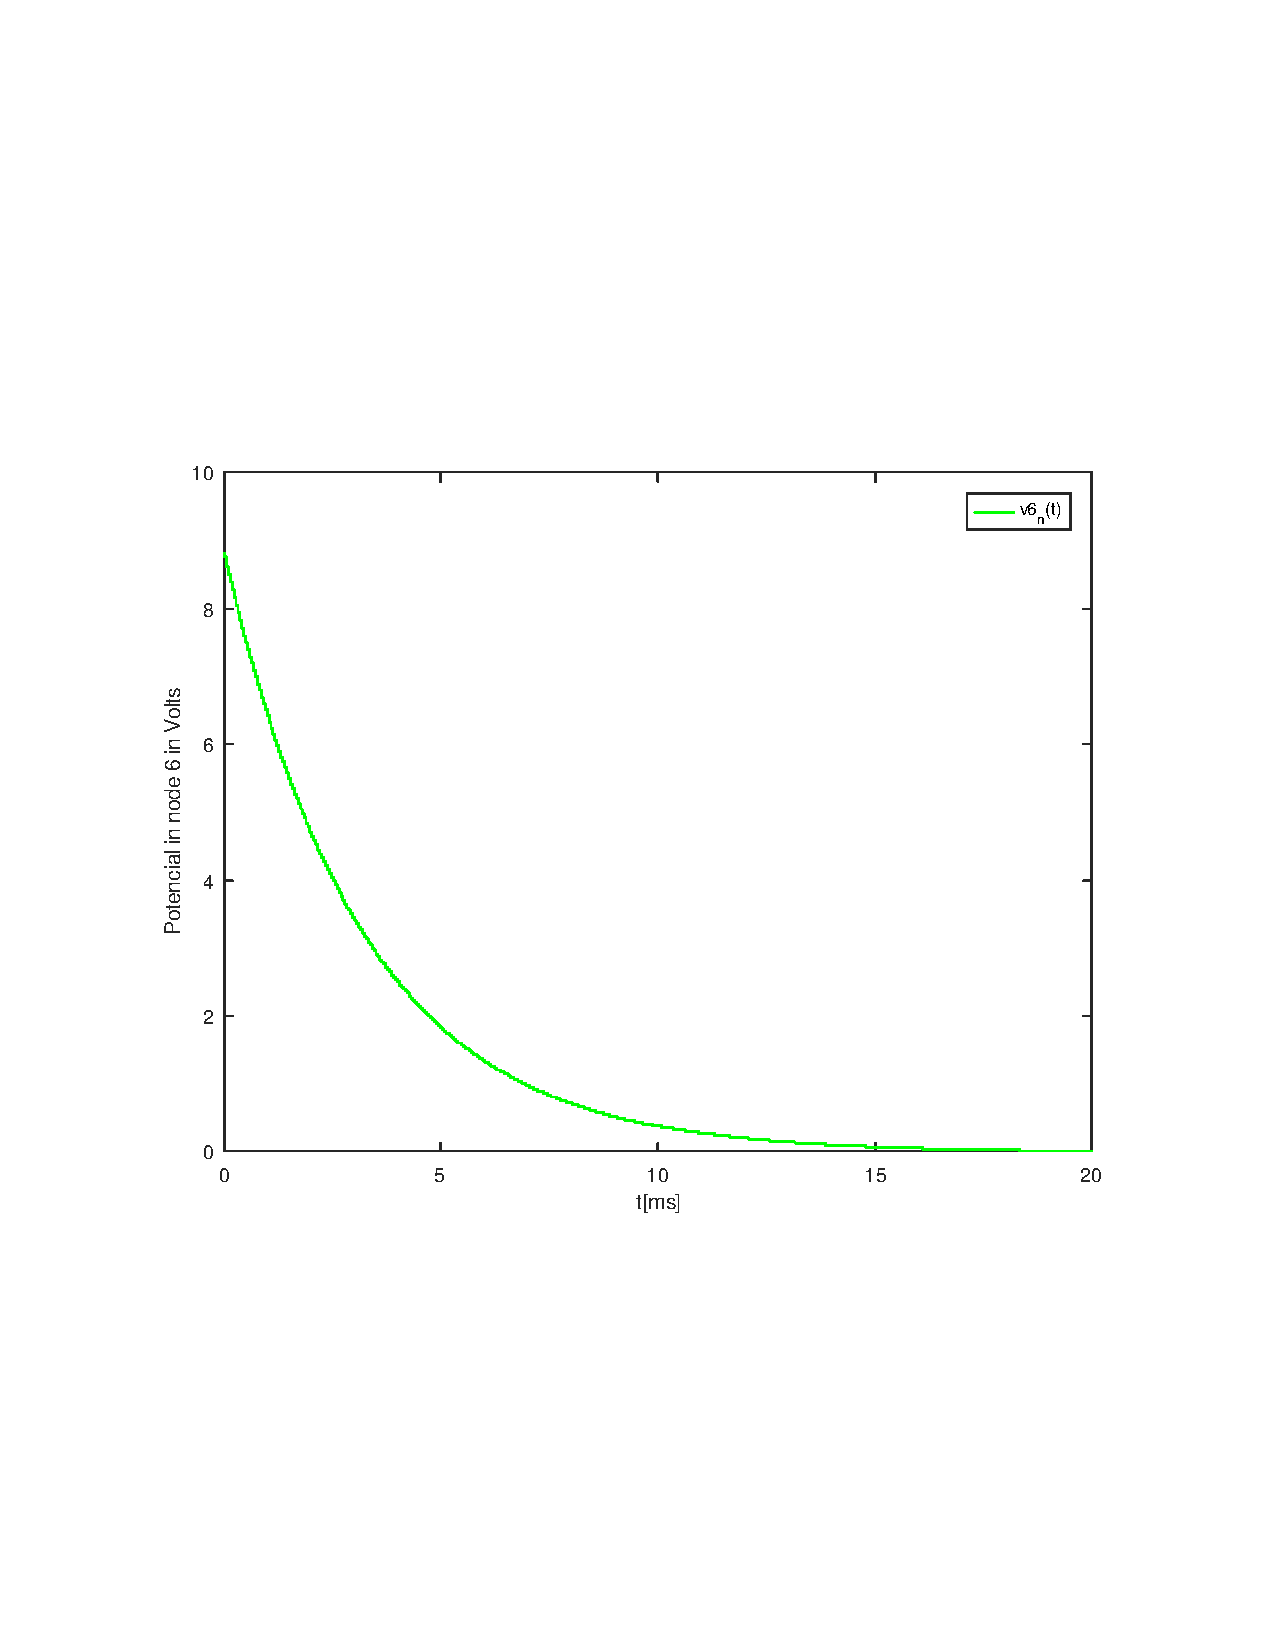
\includegraphics[width=0.9\linewidth]{natural_tab.pdf}
%\caption{Natural response of $V_6$ as a function os time in the interval from [0,20] ms}
%\label{fig:natural}
%\end{figure} 



%\begin{figure}[H] \centering
%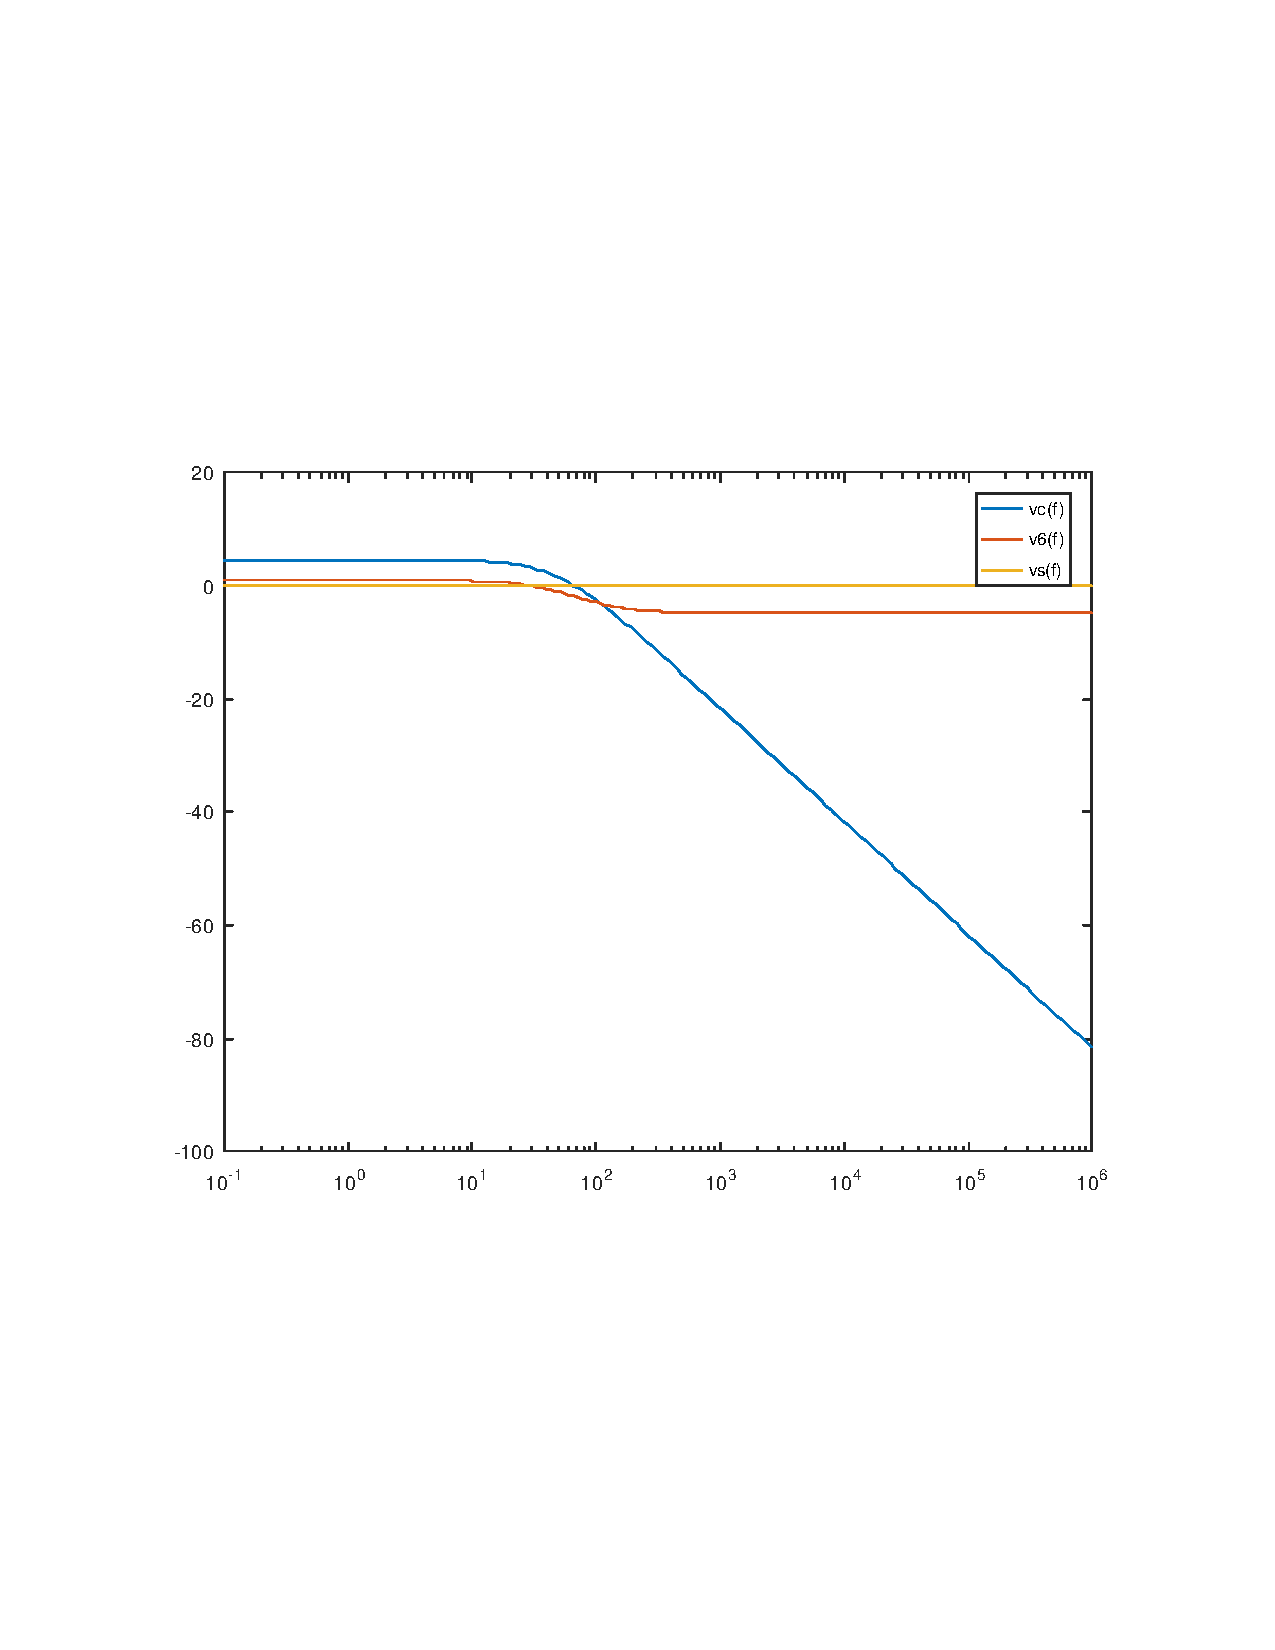
\includegraphics[width=0.9\linewidth]{freq_resp_tab.pdf}
%\caption{Graph for amplitude frequency response, in dB, of $V_c$, $V_6$ and $V_s$ for frequencies ranging from 0.1Hz to 1MHz (logarithmic scale).}
%\label{fig:freq_resp}
%\end{figure}




\pagebreak


